\chapter{Optimisation: Allocating Scarce Resources}

\begin{weekbox}
\textbf{Theme.} Prediction says what will happen; optimisation says what to do about it. Translate a decision into
variables, an objective and constraints, let a solver find the best plan, then read the shadow prices to learn what
the constraints are costing you.\\
\textbf{Outcomes.} LO6, LO1.\quad \textbf{Tools.} PuLP with CBC, OR-Tools (routing).\\
\textbf{Data.} Mboa central kitchen; 15 Cameroonian cities with approximate coordinates and populations; 13 delivery
points in Douala.\\
\textbf{Lab.} Product mix with shadow prices; national distribution-network design; cashier roster; delivery routes.\\
\textbf{Deliverable.} Model notebook with each formulation written in mathematics; \textbf{capstone checkpoint 2}.
\end{weekbox}

\begin{timetable}
0:00--0:20 & Briefing & ``Where should Mboa put its warehouses if it expands to the north?''\\
0:20--1:10 & Concepts & Formulation recipe, LP geometry and duality, integer logic, network models, routing\\
1:10--2:40 & Guided lab & Lab 5, Steps 1--4 (break at 1:55)\\
2:40--3:40 & Challenge & Exercises 5.4--5.8; capstone checkpoint 2\\
3:40--4:00 & Debrief & Each student explains one shadow price in plain language\\
\end{timetable}

\section{From a decision to a model}
An optimisation model has three parts: \textbf{decision variables} (what we control), an \textbf{objective} (what we
maximise or minimise) and \textbf{constraints} (what limits us). In general,
\[ \min_{x}\ f(x)\quad\text{subject to}\quad g_i(x)\le 0\ (i=1,\dots,m),\quad x\in X, \]
where $X$ fixes the domain (non-negative reals, integers, binaries). A plan that satisfies every constraint is
\emph{feasible}; the best feasible plan is \emph{optimal}.

\begin{keyformula}{The four-step formulation recipe}
\begin{enumerate}[nosep]
\item \textbf{Variables}: define each unknown with its unit (``$x_i$ = loaves of product $i$ baked per day'').
\item \textbf{Objective}: write profit or cost as a function of the variables; check the units (XAF).
\item \textbf{Constraints}: one line per scarce resource, demand limit, capacity or logical rule; check units on both sides.
\item \textbf{Domain}: non-negativity, integrality, binaries.
\end{enumerate}
Then solve a tiny version by hand or in a spreadsheet to check the model before scaling it up.
\end{keyformula}

\section{Linear programming}
When the objective and constraints are linear and variables continuous, the model is a linear programme (LP):
$\max\ c^\top x$ subject to $Ax\le b$, $x\ge0$. LPs with millions of variables solve in seconds.

\subsection{Geometry}
\begin{example}{A two-product LP}
A workshop makes tables ($x_1$, margin 30\,000\xaf) and chairs ($x_2$, margin 20\,000\xaf). Carpentry: $x_1+x_2\le4$
days; finishing: $x_1+3x_2\le6$; at most 3 tables. Maximise $30x_1+20x_2$ (thousand XAF).
\begin{center}
\begin{tikzpicture}
\begin{axis}[width=7.2cm,height=5.4cm,xmin=0,xmax=6.4,ymin=0,ymax=4.6,axis lines=left,xlabel={$x_1$ tables},ylabel={$x_2$ chairs},
  tick label style={font=\scriptsize},label style={font=\scriptsize}]
\addplot[fill=teal!20,draw=none] coordinates {(0,0) (3,0) (3,1) (1.5,1.5) (0,2)} -- cycle;
\addplot[navy,thick,domain=0:4.4] {4-x} node[pos=0.95,above,font=\tiny]{carpentry};
\addplot[navy,thick,domain=0:6.3] {(6-x)/3} node[pos=0.9,above,font=\tiny]{finishing};
\addplot[navy,thick] coordinates {(3,0) (3,4.4)} node[pos=0.9,right,font=\tiny]{$x_1\le3$};
\addplot[orange,dashed,thick,domain=1.8:4.6] {(110-30*x)/20};
\addplot[only marks,mark=*,mark size=2.2pt,brick] coordinates {(3,1)};
\node[font=\scriptsize,brick,anchor=west] at (axis cs:3.1,1.2) {optimum $(3,1)$, $z=110$};
\end{axis}
\end{tikzpicture}
\end{center}
The feasible region is a polygon; the objective's iso-profit lines (dashed) slide outward until they last touch it,
always at a vertex. The optimum is 3 tables and 1 chair for 110\,000\xaf. The simplex method walks from vertex to
better vertex; interior-point methods cut through the middle. HiGHS and CBC implement both.
\end{example}

\subsection{Duality and shadow prices}
Every LP has a dual: $\min\ b^\top y$ subject to $A^\top y\ge c$, $y\ge0$. At the optimum the two objective values are
equal (strong duality), and the dual variable $y_i^*$ of constraint $i$ is its \textbf{shadow price}.

\begin{definition}{Shadow price}
The shadow price of a constraint is the change in the optimal objective per unit increase in its right-hand side,
holding everything else fixed, valid within a range reported by sensitivity analysis. A constraint with slack has
shadow price zero (complementary slackness).
\end{definition}

Shadow prices answer the questions managers actually ask: \emph{what is one more kilogram of flour worth? Should we
pay overtime at 3\,000\xaf\ an hour?} If the shadow price exceeds the cost of the extra unit, buy it. The
\textbf{reduced cost} of a variable at zero is how much its margin must improve before it enters the plan.

\begin{pitfall}{Sign conventions differ between solvers}
For a maximisation, CBC reports a binding $\le$ constraint's shadow price as positive; HiGHS, through PuLP, may
report it negative. Always check one shadow price by re-solving with the right-hand side increased by one unit.
\end{pitfall}

\section{Integer programming}
Real decisions are often yes/no (open a warehouse, assign a driver) or come in whole units (vans, staff). Adding
integer variables gives a mixed-integer linear programme (MILP).

\begin{center}\small
\begin{tabularx}{\linewidth}{@{}L{4.0cm}L{5.0cm}Y@{}}
\toprule
\textbf{Logic} & \textbf{Constraint} & \textbf{Meaning}\\\midrule
Fixed charge & $q\le M\,y$, cost $F y$ & produce only if the line is set up\\
At most $k$ of $n$ & $\sum_j y_j\le k$ & choose at most $k$ projects\\
If A then B & $y_A\le y_B$ & open a DC only if its road is built\\
Either--or & $g_1(x)\le M y,\ g_2(x)\le M(1-y)$ & one of two constraints must hold\\
Linking & $a_{fc}\le y_f$ & serve city $c$ from $f$ only if $f$ is open\\\bottomrule
\end{tabularx}
\end{center}
Choose $M$ as small as the problem allows: a huge big-$M$ makes the LP relaxation weak and the solver slow.

\paragraph{Branch and bound} The solver first drops integrality and solves the LP relaxation, which gives a
\emph{bound}. If a variable is fractional, it branches ($y\le0$ or $y\ge1$), solving two LPs, and prunes branches whose
bound is worse than the best integer plan found. The \textbf{optimality gap}, $(\text{bound}-\text{best})/\text{best}$,
says how far from optimal the current plan can be. For large models, stopping at a 1\% gap is usually wiser than
waiting hours for a proof.

\section{Network and location models}
\paragraph{Transportation} Ship from supplies $s_i$ to demands $d_j$ at unit cost $c_{ij}$:
$\min\sum c_{ij}x_{ij}$ s.t.\ $\sum_j x_{ij}\le s_i$, $\sum_i x_{ij}=d_j$, $x\ge0$. Its LP solution is automatically
integer when supplies and demands are integers.

\paragraph{Assignment} Assign $n$ workers to $n$ jobs, each once, at minimum cost: a transportation problem with all
supplies and demands equal to one.

\paragraph{Capacitated facility location} Choose which facilities to open ($y_f$) and which city each serves
($a_{fc}$):
\[
\min \sum_f F_f y_f + \sum_{f,c} t_{fc}\,d_c\,a_{fc}
\quad\text{s.t.}\quad \sum_f a_{fc}=1\ \forall c,\quad \sum_c d_c a_{fc}\le C_f y_f\ \forall f,\quad a_{fc}\le y_f,\quad y\in\{0,1\}.
\]
This is the model behind every ``where should we put the warehouse'' study, and the core of Lab 5.

\section{Scheduling and routing}
\paragraph{Workforce scheduling} Staff work five consecutive days and rest two. Let $n_p$ be the number starting on
day $p$; each day's requirement $r_d$ must be covered: $\sum_{p:\,d\in\text{shift}(p)} n_p\ge r_d$. Minimise
$\sum_p n_p$. The requirements come from the forecast (Week 3) converted to staff by a service standard (Week 6):
the whole decision thread in one model.

\paragraph{Vehicle routing (VRP)} Visit every customer once with a fleet of capacitated vehicles starting and ending at
a depot, minimising distance. Exact MILP formulations work for a few dozen customers; real problems use heuristics
and local search, which OR-Tools provides with time windows, capacities and driver breaks.

\begin{realcase}{UPS ORION}
UPS's ORION system (On-Road Integrated Optimization and Navigation) re-optimises the daily route of each delivery
driver. After its US roll-out in 2016 UPS reported savings of about 100 million miles and 10 million gallons of fuel a
year. Two lessons from published accounts: the routes had to respect drivers' knowledge and customers' habits to be
adopted, and small savings per stop (a mile per driver per day) add up to tens of millions of dollars at scale.
\end{realcase}

\begin{insight}{Predict-then-optimise, and its limits}
Most plans in practice feed a point forecast into an optimiser. That works when the plan is cheap to adjust. When it is
not (a warehouse, a December order), the forecast's uncertainty must enter the optimisation itself. Week 6 shows how,
and measures how much it is worth.
\end{insight}

% ------------------------------------------------------------------ LAB
\section{Practical Lab 5: Four allocation decisions}
\begin{labbox}{Practical lab --- PuLP and OR-Tools}
\textbf{Goal.} Formulate, solve and interpret four models of increasing realism. For each, write the mathematics in a
Markdown cell before coding. \textbf{Data.} Defined in the code; city coordinates and populations are approximate and
rounded, for teaching (replace with BUCREP census data and OpenStreetMap road distances in real work).
\textbf{Time.} 90 minutes.
\end{labbox}

\step{Step 1: Product mix and shadow prices}
\codeout{lab5_s1}{Mboa central kitchen: three products, three resources, three demand caps.}
\interp{The kitchen sells all the beignets and meat pies it can and uses the remaining flour for bread (640 loaves).
Flour is the binding resource: its shadow price is 240\xaf\ per kg, so buying extra flour at up to 240\xaf\ above its current
cost raises margin. Oven time and labour have slack and are worth nothing at the margin: overtime for bakers would
waste money. The demand caps on beignets (13\xaf) and meat pies (156\xaf) say that one more unit of meat-pie demand,
through marketing for example, is worth 156\xaf, because it would use flour taken from bread.}

\step{Step 2: Where to put distribution centres in Cameroon}
\codeout{lab5_s2}{Capacitated facility location with an inbound leg from the port of Douala.}
\interp{At 90\xaf\ per tonne-km the model opens Douala and Bafoussam, with total weekly cost 14.7\,M\xaf. Serving
Yaoundé from Bafoussam surprises most students: the model trades about 2\,M\xaf\ a week of extra fixed cost for a
Yaoundé site against the longer haul, and the haul is cheaper at this freight rate. At 120\xaf\ per tonne-km or more,
Douala and Yaoundé is optimal. The decision depends on a number nobody knows precisely, so the recommendation is a
\emph{range}: if freight is expected to exceed about 100--120\xaf\ per tonne-km over the life of the lease, choose
Yaoundé. A first version of this model without the inbound leg from the port kept Douala closed and served the port city from inland. That
version was wrong.}

\begin{pitfall}{Forgetting a cost leg}
Every cost the decision changes must be in the objective. Our first model omitted the inbound freight from the port,
where most goods enter Cameroon, and so preferred inland sites. When a solution surprises you, check what the model
does \emph{not} know before trusting or rejecting it.
\end{pitfall}

\step{Step 3: A cashier roster from the forecast}
\codeout{lab5_s3}{Five-days-on, two-off cyclic roster covering daily requirements.}
\interp{Eleven cashiers cover the week, which equals the lower bound $\lceil 58/5\rceil$, so no roster can do better.
Two cashier-days of surplus fall on Wednesday and Thursday, a good time for training or stock counts. The requirement row
is the interface with Weeks 3 and 6: change the forecast or the service standard and the roster follows.}

\step{Step 4: Delivery routes in Douala}
\codeout{lab5_s4}{Capacitated vehicle routing with OR-Tools and guided local search (5-second limit).}
\begin{figure}[H]\centering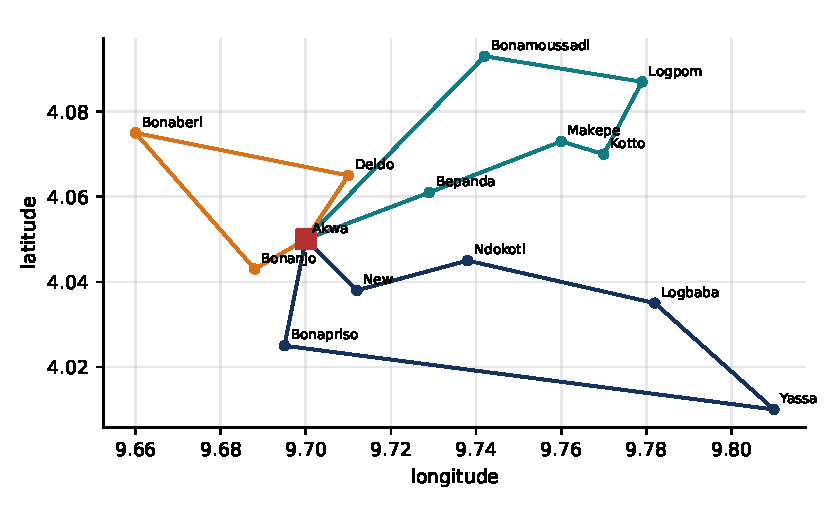
\includegraphics[width=0.66\linewidth]{../figs/lab5_vrp.pdf}
\caption{Three van routes from the Akwa depot (square). Coordinates are approximate.}\end{figure}
\interp{Three vans cover 13 sites in 91\,km; two vans are nearly full (34 and 35 of 35 crates), one half-loaded.
The half-empty van suggests asking whether a cheaper vehicle, or two trips by one van, would serve the
Bonabéri side. Distances here are straight lines times 1.4; Douala traffic means time, not distance, is the real
cost, which OR-Tools handles with a time dimension and time windows.}

\paragraph{So what (model answer)} \emph{Flour, not labour or ovens, limits the kitchen: each extra kilogram is
worth 240\xaf. For national expansion, open Douala plus Bafoussam if freight stays below about 100\xaf\ per tonne-km,
otherwise Douala plus Yaoundé; the difference is 2--4\,M\xaf\ a week. Eleven cashiers on a five-and-two roster cover
Douala Akwa's forecast demand with no waste.}

% ------------------------------------------------------------------ EXERCISES
\section{Exercises}
\begin{enumerate}[label=\textbf{5.\arabic*},leftmargin=2.4em]
\item \emph{(Hand solution)} Solve the table--chair LP graphically with the chair margin raised to 40\,000\xaf. Which
vertex is optimal now? Compute the dual prices of carpentry and finishing.
\item \emph{(Duality)} Write the dual of the kitchen LP in Step 1 and verify that its optimal value equals 275\,400\xaf.
\item \emph{(Modelling logic)} Add to Step 1: meat pies need a refrigerated line costing 40\,000\xaf\ a day if used at all.
Formulate with a binary variable and re-solve. Does the plan change?
\item \emph{(Sensitivity)} In Step 1, increase flour from 400 to 500\,kg in steps of 20. Plot margin against flour. Where
does the shadow price change, and why?
\item \emph{(Location)} In Step 2, allow split sourcing (\texttt{single\_source=False}). How much cheaper is it, and why
might managers still prefer single sourcing?
\item \emph{(Location)} Add a third candidate size: a ``hub'' in Douala with capacity 300\,t at 7\,M\xaf\ a week. Re-solve
for freight rates 60--150\xaf.
\item \emph{(Roster)} Add part-time cashiers working Friday to Sunday only, at 45\% of a full-timer's cost. Formulate and
solve. How many full-timers remain?
\item \emph{(Routing)} Add time windows: Bonanjo offices accept deliveries only 8:00--10:00. Use an OR-Tools time dimension
with 25\,km/h average speed and 15 minutes per stop.
\end{enumerate}

\section{Take-home assignment 5 and capstone checkpoint 2}
\begin{enumerate}[nosep]
\item Mboa is considering a cold-chain DC for fresh products (bread, eggs). Extend the Step 2 model with product-specific
capacities and a maximum delivery distance of 300\,km for fresh goods. Write a one-page recommendation with the cost of
the fresh-distance rule.
\item \textbf{Checkpoint 2} (in class): your capstone's model or decision prototype running on real data, compared with
the baseline from checkpoint 1, with a first estimate of the XAF impact.
\end{enumerate}
